\documentclass[letterpaper]{article}
\usepackage{multicol} 
\usepackage{graphicx}
\usepackage[utf8]{inputenc}
\usepackage{fancyhdr}
\usepackage{setspace}
\usepackage{amsmath}
\usepackage{mathtools}
\usepackage{pifont}
\usepackage{enumerate}
\usepackage{enumitem}
\usepackage{amssymb}
\usepackage{anysize}
\usepackage{listings}
\usepackage{color}
\usepackage[margin=2cm,bmargin=3cm,headsep=.1cm]{geometry}
\usepackage{indentfirst}
\usepackage[labelfont=bf]{caption}
\usepackage[font={small,it}]{caption}
\usepackage{hyperref}

\renewcommand{\figurename}{Figura}

%Color
\usepackage{color}
\definecolor{nc1}{RGB}{16, 89, 82}
\definecolor{nc2}{RGB}{23, 127, 117}
\definecolor{nc3}{RGB}{33, 162, 168}
\usepackage{sectsty}
\sectionfont{\color{nc1}}
\subsectionfont{\color{nc2}}
\subsubsectionfont{\color{nc3}}


\definecolor{codegreen}{rgb}{0,0.6,0}
\definecolor{codegray}{rgb}{0.5,0.5,0.5}
\definecolor{codepurple}{rgb}{0.58,0,0.82}
\definecolor{backcolour}{rgb}{0.95,0.95,0.92}
 
\lstdefinestyle{mystyle}{
    backgroundcolor=\color{backcolour},   
    commentstyle=\color{codegreen},
    keywordstyle=\color{magenta},
    numberstyle=\tiny\color{codegray},
    stringstyle=\color{codepurple},
    basicstyle=\footnotesize,
    breakatwhitespace=false,         
    breaklines=true,                 
    captionpos=b,                    
    keepspaces=true,                 
    numbers=left,                    
    numbersep=5pt,                  
    showspaces=false,                
    showstringspaces=false,
    showtabs=false,                  
    tabsize=2
}
 
\lstset{style=mystyle}
\sloppy
\pagestyle{fancy}
\marginsize{3cm}{3cm}{2cm}{2cm}
\fancyfoot[C]{\thepage}%numero de pagina en el centro abajo
\setlength{\headheight}{46pt}
\renewcommand{\headrulewidth}{0pt}


\newcommand{\imagen}[2]
{
\begin{center}
{\includegraphics[width=\textwidth]{#1}}
\begin{spacing}{0.7}
{\footnotesize{#2}}
\end{spacing}
\end{center}
}

\newcommand{\5}
{
\\[.5cm]
}


\setenumerate{label= \textbf{\alph*)}}
\setenumerate[2]{label= \textbf{\arabic*.}}
\setenumerate[3]{label*= \textbf{\arabic*.}}

\begin{document}


\begin{titlepage}


\begin{center}


\includegraphics[width=4cm,height=3cm]{logo-usm}
\\[1.0cm]


\textsc{\Large Universidad Técnica Federico Santa María \\[0.5cm] Campus San Joaquín}
\\[1.0cm]


\noindent\rule{16cm}{0.4pt}
\\[0.5cm]
    {\textsc{\Large Laboratorio 3 y 4 - CC2 - 2015-2}}
\\[0.5cm]
\noindent\rule{16cm}{0.4pt}
\\[0.5cm]


\begin{minipage}{1.0\textwidth}
\center{\textsc{Felipe Morales - Rol: 201273564-5 - felipe.morales.12@sansano.usm.cl}}


\end{minipage}

\end{center}
\end{titlepage}

%\\\\\\\\\\\\\\\\\\\\\\\\\\\\\\\\\\\\\\\\\\\\\\\\\\\\
% 				DESCRIPCION LABORATORIO				|
%////////////////////////////////////////////////////
\newpage
\section{Descripción Laboratorio}
El presente informe contiene el desarrollo de los laboratorios 3 y 4. \\[0.2cm]

En el laboratorio 3 se realizará una implementación del método de diferencias finitas para la resolución de ecuaciones diferenciales parciales (EDP) clasificadas como elípticas y parabólicas. Las ecuaciones elípticas son aquellas que no dependen del tiempo y cuyo discriminante es menor a 0 ($B^2-4AC < 0$). Por otro lado, las ecuaciones parabólicas evolucionan en el tiempo y su discriminante es igual a 0 ($B^2-4AC = 0$). \\[0.2cm]

Se realizará también un análisis de los parámetros necesarios para obtener resultados óptimos usando dichos algoritmos y cuales son sus limitaciones en su utilización. \\[0.2cm]

Cabe notar que el discriminante se obtiene analizando la estructura de la EDP de la forma 
\begin{equation}
AU_{xx} + BU_{xy} + CU_{yy} + F(U_x, U_y, U, x, y) = 0
\end{equation}
En el laboratorio 4 se realizará una simulación de una ecuación de onda en dos dimensiones, que corresponde a una ecuación en derivadas parciales de tipo hiperbólica. Estas EDP se caracterizan por tener como condición inicial la derivada temporal de primer orden, en contraste con las otras dos en donde solo se necesitaban condiciones iniciales de la función original. Estas ecuaciones poseen un discriminante positivo ($B^2-4AC > 0$).

%\\\\\\\\\\\\\\\\\\\\\\\\\\\\\\\\\\\\\\\\\\\\\\\\\\\\
% 					RESULTADOS						|
%////////////////////////////////////////////////////
\newpage
\section{Desarrollo y análisis de resultados}
A continuación se presentan las respuestas a las preguntas del laboratorio con su respectivo análisis.
\subsection{Parte 1: Laboratorio 3}
\subsubsection{EDP Elíptica}
\begin{itemize}
	\item[a)] La implementación del algoritmo de las diferencias finitas se basa en ecuaciones diferenciales de la forma:
    \begin{equation}
    \begin{split}
    	U_{xx}(x, y) + U_{yy}(x, y) = f(x, y) + Z(x, y) U(x, y) \\
        U(x, Y_{min}) = down(x) \\
        U(x, Y_{max}) = up(x) \\
        U(X_{min}, y) = left(y) \\
        U(X_{max}, y) = right(y) \\
        X_{min} < x < X_{max} \\
        Y_{min} < y < Y_{max} \\
    \end{split}
	\end{equation}
    
    A partir de la ecuación 2, se puede realizar una aproximación de las segundas derivadas haciendo uso de central difference para derivadas de segundo orden, y considerando una distancia entre puntos para la discretización de $\Delta x$ y $\Delta y$. Entonces, la ecuación queda:
    \begin{equation}
    \begin{split}
    \frac{U(x + \Delta x, y)-2U(x, y) + U(x - \Delta x, y)}{\Delta x} + \frac{U(x, y + \Delta y ) - 2U(x, y) + U(x, y - \Delta y)}{\Delta y} - \\Z(x, y) U(x,y) = f(x, y)
    \end{split}
    \end{equation}
    
    Luego, discretizando la ecuación 3 en donde $W_{i,j}$ representa al punto $(i \cdot \Delta x, j \dot \Delta y)$, tenemos:
    \begin{equation}
    	\frac{W_{i-1,j} - 2W_{i, j} + W_{i+1, j}}{\Delta x} + \frac{W_{i, j-1} - 2W_{i, j} + W_{i, j+1}}{\Delta y} - Z(i \cdot \Delta x, j \cdot \Delta y)W_{i, j} = f(i \cdot \Delta x, j \cdot \Delta y)
    \end{equation}
    
    La cual se puede traducir a un sistema lineal. El algoritmo que se implementará resolver todos los puntos utilizando una nueva notación. Además, esta notación sirve para evadir tener un conflicto de índices en dicho sistema lineal. Para obtener la notación, se re-etiquetan los puntos de la forma $v_{i + (j-1)m} = W_{i, j}$ en donde $m$ corresponde al numero total de puntos en el eje Y, y se introducen las condiciones iniciales, como se puede observar a continuación:
    \begin{equation}
    \begin{split}
    W_{i,0} = U(x_i, Y_{min}) = down(x_i), i \in \{0,1,...,N_x\} \\
    W_{N_x,j} = U(X_{max}, y_j) = right(y_i), j \in \{0,1,...,N_y\} \\
    W_{i,N_y} = U(x_i, Y_{max}) = up(x_i), i \in \{0,1,...,N_x\} \\
    W_{0,j} = U_(X_{min}, y_j) = left(y_i), j \in \{0,1,...,N_y\}
    \end{split}
	\end{equation}
    Considerando $X_{min} < x < X_{max}$ y $Y_{min} < y < Y_{max}$, la discretización en la ecuación 4 y el cambio de variable para etiquetar mencionado. \\[0.2cm]
    
    A continuación, se presenta la implementación del algoritmo de diferencias finitas:
    
    
\begin{lstlisting}[language=Python]
#Diferencias finitas para EDP eliptica. (Nota: Xmin < Xmax, Ymin < Ymax)
#F: Funcion F(x, y) que esta a la derecha de la ecuacion.
#Z: Funcion Z(x, y)  que acompana al termino u(x, y) en la ecuacion (si es de helmholtz)
#Xmin: Limite inferior x
#Xmax: Limite superior x
#Ymin: Limite inferior y
#Ymax: Limite superior y
#Nx: Puntos requeridos eje x (h = (Xmax-Xmin)/Nx)
#Ny: Puntos requeridos eje y (k = (Ymax-Ymin)/Ny)
#up: condicion inicial arriba u(x, Ymax) = up(x)
#down: condicion inicial abajo u(x, Ymin) = down(x)
#left: condicion inicial izquierda u(Xmin, y) = left(y)
#right: conidicion inicial derecha u(Xmax, y) = right(y)
#
#Return: retorna una matriz de puntos aproximados y los intervalos para los ejes X e Y
def ElipticFiniteDifference(F, Z, Xmin, Xmax, Ymin, Ymax, Nx, Ny, up, down, left, right):
	#Discretizacion en x e y, o bien, creacion de particiones.
	x = np.linspace(Xmin, Xmax, Nx+1)
	y = np.linspace(Ymin, Ymax, Ny+1)

	#Definicion de step size, o bien, distancia entre los puntos
	#de la discretizacion.
	H = x[1]-x[0]
	K = y[1]-y[0]

	#Crear matrices del sistema lineal.
	mn = (Nx+1)*(Ny+1)
	A = np.zeros([mn, mn])
	b = np.zeros([mn, 1])

	#Matriz para la obtencion de los indices
	def index(i, j, m=Nx+1):
		return j + i*m

	#Diferencias finitas, llenado de la matriz
	for i in xrange(Nx+1):
		for j in xrange(Ny+1):

			#Obtencion del indice actual.
			k = index(i, j)

			#Esta en la frontera up
			if j == Ny:
				A[k, k] = 1
				b[k] = up(x[i])

			#Esta en la frontera down
			elif j == 0:
				A[k, k] = 1
				b[k] = down(x[i])

			#Esta en la frontera left
			elif i == 0:
				A[k, k] = 1
				b[k] = left(y[j])

			#Esta en la frontera right
			elif i == Nx:
				A[k, k] = 1
				b[k] = right(y[j])
			else:
				#Resto de los puntos desconocidos
				A[k, k] = -2/H**2 -2/K**2 -Z(x[i], y[j])
				A[k, index(i+1, j)] = 1/H**2
				A[k, index(i-1, j)] = 1/H**2
				A[k, index(i, j-1)] = 1/K**2
				A[k, index(i, j+1)] = 1/K**2
				b[k] = F(x[i], y[j])
	w = np.linalg.solve(A, b)
	return w, x, y
\end{lstlisting}

\item[b)] A continuación se adjuntan los gráficos para las 3 funciones propuestas, utilizando valores de $h$ igual a 0.1, 0.05 y 0.01, donde $\Delta y = \Delta x = h$:

	\begin{itemize}
    	\item[i)] Para la ecuación diferencial parcial 1 ($U_{xx}(x,y)+U_{yy}(x,y)-\sin(\pi x y) - (x^2+ y^2)U(x,y) = 0$):
        \begin{center}
        	\centerline{%
            	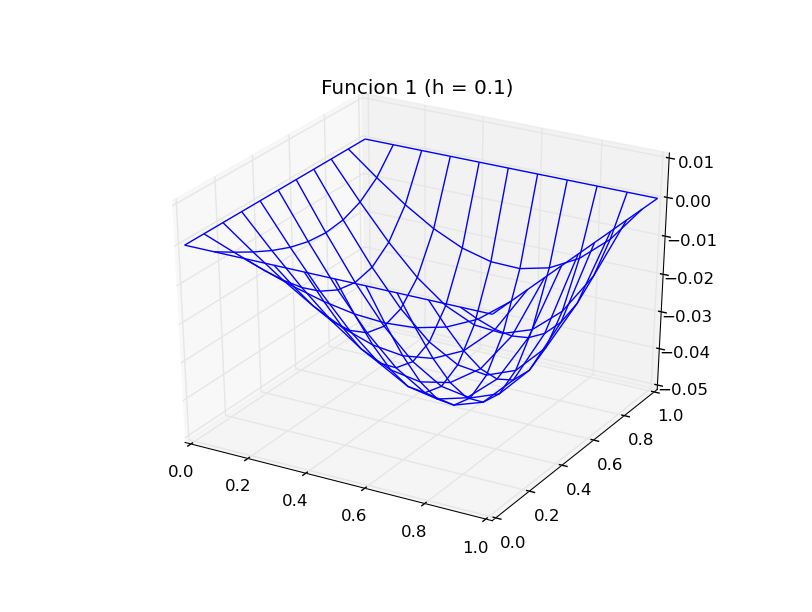
\includegraphics[scale=0.4]{f1_a}%
            	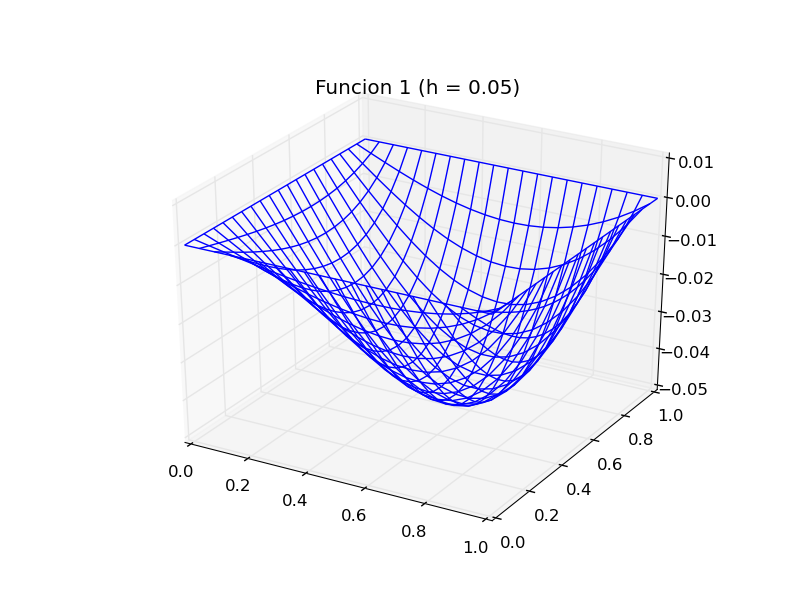
\includegraphics[scale=0.4]{f1_c}%
            }%
            \centerline{%
            	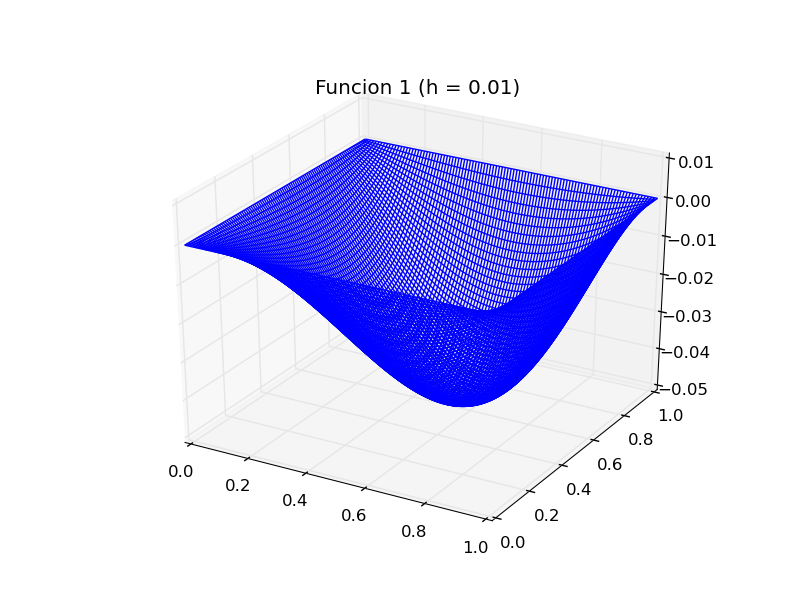
\includegraphics[scale=0.4]{f1_b}%
              	\hspace{0.5\linewidth}  
            }%
        \end{center}
        
        \item[ii)] Para la ecuación diferencial parcial 2 ($U_{xx}(x,y)+U_{yy}(x,y)-\cos(\pi x y)-e^{2xy} = 0$):
        \begin{center}
        	\centerline{%
            	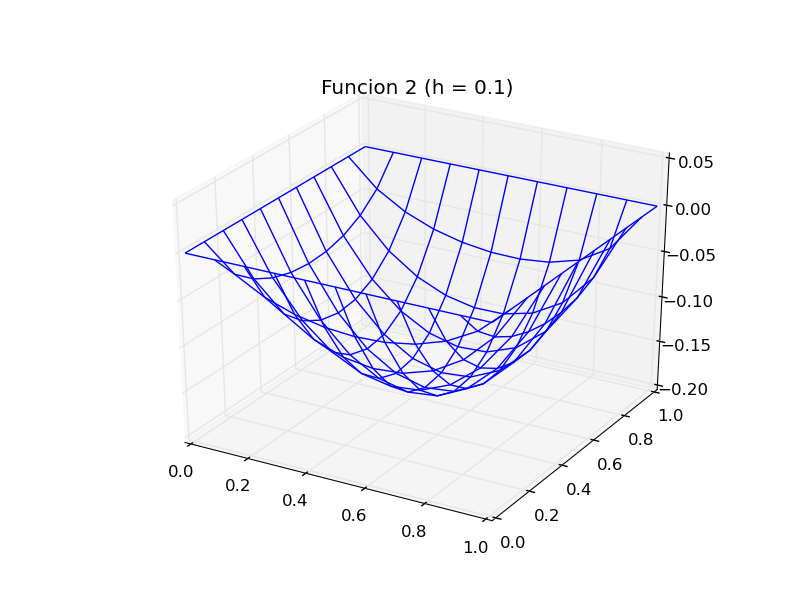
\includegraphics[scale=0.4]{f2_a}%
            	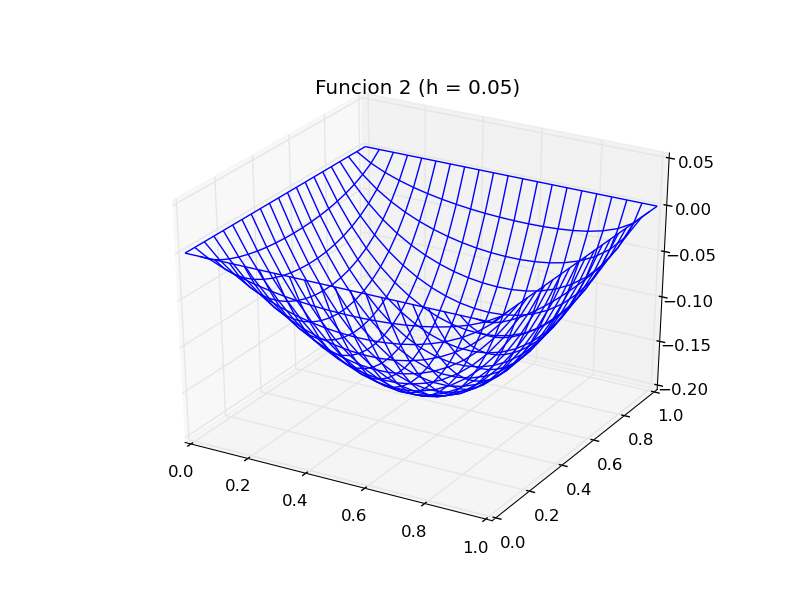
\includegraphics[scale=0.4]{f2_c}%
            }%
            \centerline{%
            	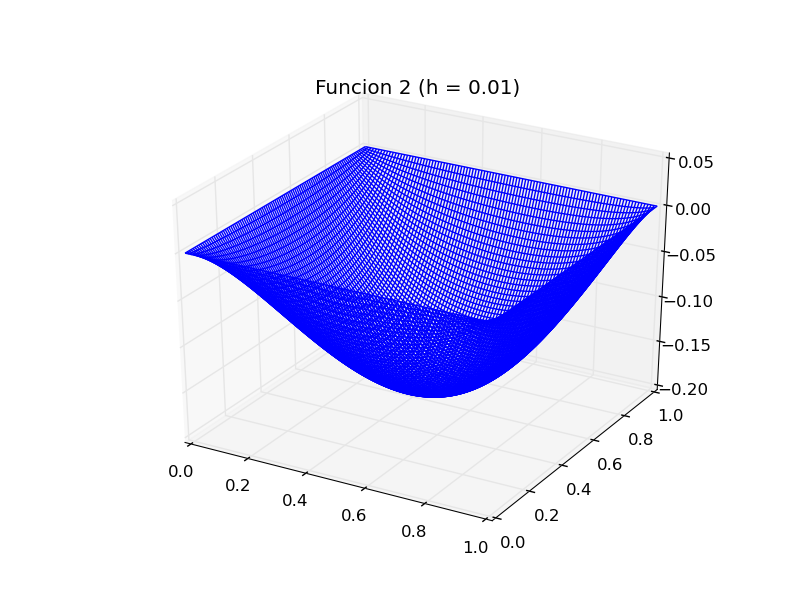
\includegraphics[scale=0.4]{f2_b}%
                \hspace{0.5\linewidth}
            }%
        \end{center}
        
        \item[iii)] Para la ecuación diferencial parcial 3 ($U_{xx}(x,y)+U_{yy}(x,y) = x$) :
        \begin{center}
        	\centerline{%
            	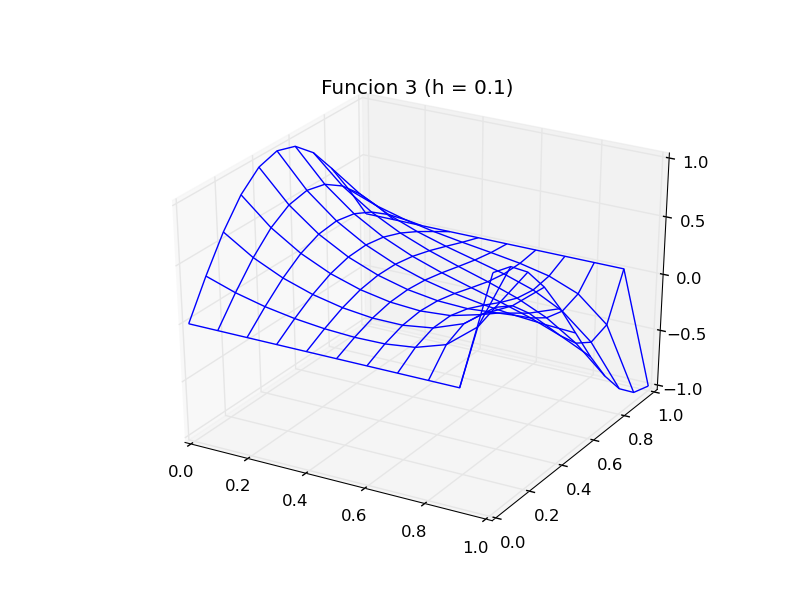
\includegraphics[scale=0.4]{f3_a}%
            	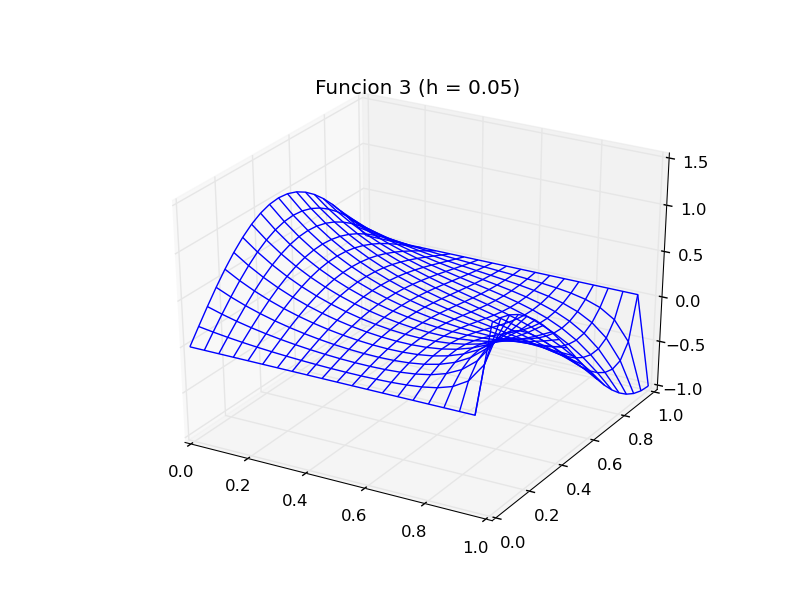
\includegraphics[scale=0.4]{f3_c}%
            }%
            \centerline{%
            	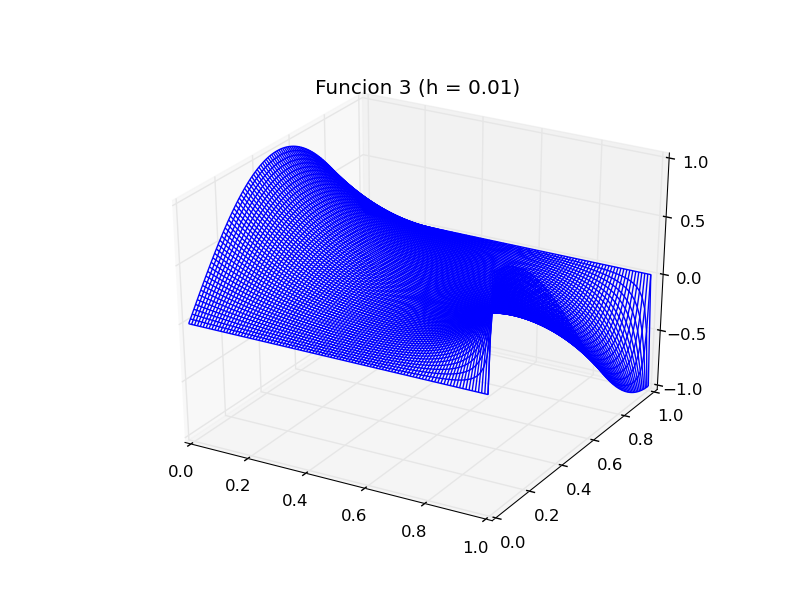
\includegraphics[scale=0.4]{f3_b}%
                \hspace{0.5\linewidth}
            }%
        \end{center}
	\end{itemize}
 \item[c)] En primera instancia, se puede notar que a medida que se aumenta el valor de $h$, aumenta así la precisión de los gráficos obtenidos con el algoritmo. Lo anterior es bastante intuitivo considerando que con un mayor valor de $h$, se tendrá una mayor cantidad de puntos disponibles para graficar. Sin embargo, a medida que aumenta el valor de h, también aumenta la cantidad de memoria requerida para resolver el sistema lineal, así como también el tiempo requerido para realizar la computación de los sistema lineales. Ya con valores cercanos a $h = 0.001$ es imposible realizar la computación en computadores promedio debido a problemas de memoria. Sin embargo, en el caso de que no existiesen aquellas limitaciones de computo, se pueden seleccionar $\Delta x$ y $\Delta y$ cualesquiera, ya que no existen condiciones de estabilidad. \\[0.2cm]
 Las EDP Elípticas permiten modelar fenómenos en donde la variable tiempo es inexistente y en donde solo se depende de la posición en el eje X e Y (en el caso de 2 dimensiones). Un ejemplo es la ecuación de Schrödinger la cual describe la evolución temporal de una partícula masiva no relativista. \\[0.2cm]
 En el primer y segundo gráfico, se puede notar que a medida que nos acercamos al centro de la malla en el deje X e Y, disminuye rápidamente el valor de $U(x, y)$hacia valores negativos. Por otro lado, la función 3 presenta un comportamiento diferente en donde se tienen valores superiores e inferiores a $U(x, y) = 0$. \\[0.2cm]
 Lo anterior se explica debido a que las condiciones iniciales para las funciones 1 y 2 son nulas, mientras que la función 3 tiene condiciones iniciales especificas. Son estas condiciones iniciales las que indican como se comportan la función en sus extremos, modificando así, la estructura y forma completa de la figura final. Otro factor importante es la función a la que está igualada la EDP, siendo ésta última la que ejerce la mayor influencia en el comportamiento de los puntos que no están en la frontera de la región. \\[0.2cm]
 El error de aproximación del método esta relacionado con las diferencias finitas. Si consideramos que el error para la diferencia finita de segundas derivadas para una función arbitraria $f(x)$ corresponde a $O(\Delta x^2)$, tenemos entonces un error final de $O(\Delta x^2) + O(\Delta y^2)$.
\end{itemize}

\subsubsection{EDP Parabólica}
\begin{itemize}
\item[a)] La implementación del algoritmo de diferencias finitas utilizando el esquema de Crank Nicholson se realizó teniendo en cuenta una EDP parabólica de la forma:
\begin{equation}
\begin{split}
 U_{t}(x, y) = D U_{xx}(x, t) + b U_x(x, t) \\
 U(x, 0) = f(x) \\
 U(X_{min}, t) = l(t) \\
 U(X_{max}, t) = r(t) \\
 0 < t < T_{max} \\
 X_{min} < x < X_{max} \\
 \end{split}
\end{equation}

Utilizando el esquema de Crank Nicholson y utilizando central difference para el término $U_x(x, t)$ y forward difference para el término $U_t(x, t)$, obtenemos la siguiente discretización:

\begin{equation}
\begin{split}
	\frac{W_{i, n+1} - W_{i, n}}{\Delta t} = \frac{D}{2\Delta x^2} \cdot (W_{i-1, n} - 2W_{i, n} + W_{i+1, n} + W_{i-1, n+1} - 2W_{i, n+1} + W_{i+1, n+1}) + \\ 
	\frac{b}{\Delta x}(W_{i+1, n} - W_{i-1, n})
\end{split}
\end{equation}


Lo cual, con álgebra común nos queda como:
\begin{equation}
	-\sigma W_{i-1, n+1} + (2 - 2 \sigma)W_{i, n+1} -\sigma W_{i+1, n+1} = (\sigma - \beta)W_{i-1, n} + (2 + 2\sigma)W_{i, n} + (\sigma + \beta)W_{i+1, n} 	
\end{equation}

En donde $\sigma = \frac{D \Delta t}{{\Delta x}^2}$ y $\beta = \frac{b \Delta t}{\Delta x}$. \\

A partir de la discretización de la ecuación 8, es posible traducir a un sistema lineal y matricial del tipo $Ax = b$ y obtener el vector $x$ que representará la obtención de todos los puntos de $t_{n+1}$dado un tiempo $t_{n}$. \\

Así entonces, para obtener $x$ debemos resolver el sistema lineal dada la información de los puntos en el tiempo $t_n$, como sigue:
\begin{equation}
	\begin{bmatrix}
    1       & 0 & \cdots & \cdots & \cdots & 0 \\
    -\sigma       & 2-2\sigma & -\sigma & \cdots & \cdots & 0 \\
    0 & -\sigma       & 2-2\sigma & -\sigma & \cdots & 0 \\
    \cdots & \cdots & \cdots & \cdots  & \cdots & 0\\
    0 & \cdots & \cdots & \cdots  & 0 & 1 \\
	\end{bmatrix}
	\begin{bmatrix}
    W_{0, n+1} \\
    W_{1, n+1} \\
    \vdots \\
    \vdots \\
    W_{N_{x}, n+1} \\
    \end{bmatrix}
= b
\end{equation}

En donde $b$ viene dado por:
\begin{equation}
	b =
    \begin{bmatrix}
    0       & 0 & \cdots & \cdots & \cdots & 0 \\
    \sigma - \beta       & 2+2\sigma & \sigma + \beta & \cdots & \cdots & 0 \\
    0 & \sigma - \beta       & 2+2\sigma & \sigma + \beta & \cdots & 0 \\
    \cdots & \cdots & \cdots & \cdots  & \cdots & 0\\
    0 & \cdots & \cdots & \cdots  & 0 & 0 \\
	\end{bmatrix}
    \begin{bmatrix}
    W_{0, n} \\
    W_{1, n} \\
    \vdots \\
    \vdots \\
    W_{N_{x}, n} \\
    \end{bmatrix}
   +
   \begin{bmatrix}
    l(t_{n+1}) \\
    0 \\
    \vdots \\
    0 \\
    r(t_{n+1}) \\
    \end{bmatrix}    
\end{equation}
Y en donde además, se tiene que para $t_0$:
\begin{equation}
	W_0 =
    \begin{bmatrix}
    W_{0, 0} \\
    W_{1, 0} \\
    \vdots \\
    W_{N_x-1, 0} \\
    W_{N_x, 0} \\
    \end{bmatrix} 
    =
    \begin{bmatrix}
    f(0) \\
    f(\Delta x) \\
    \vdots \\
    f( (N_x-1) \cdot \Delta x) \\
    f(N_x \cdot \Delta x) \\
    \end{bmatrix} 
\end{equation}
En donde la función $f(x)$ viene dada por las condiciones iniciales en la ecuación 6. \\

Teniendo las consideraciones anteriores, se prosiguió a implementar el algoritmo:

\begin{lstlisting}[language=Python]
#Diferencias finitas para EDP parabolica. (Nota: Xmin < Xmax)
#D: Constante D que acompana al termino Uxx(x, y)
#b: Constante b que acompana al termino Ux(x, y)
#Xmin: Limite inferior x
#Xmax: Limite superior x
#Tmax: Maximo tiempo a evolucionar la solucion
#dx: Distancia entre los puntos discretizados para el eje x
#dt: Distancia entre los puntos discretizados para el eje t
#f: Condicion inicial U(x, 0) = f(x)
#l: Condicion inicial U(Xmin, t) = l(t)
#r: condicion inicial U(Xmax, t) = r(t)
#Return: retorna una matriz de puntos aproximados y los intervalos para los ejes X e Y

def CrankNicholsonFiniteDifference(D, b, Xmin, Xmax, Tmax, dx, dt, f, l, r):
	Nx = int(mt.ceil((Xmax-Xmin)/dx))
	Nt = int(mt.ceil(Tmax/dt))

	sigma = D*dt/dx**2
	beta = b*dt/dx

	W = np.zeros([Nt+1, Nx+1])

	x = np.linspace(Xmin, Xmax, Nx+1)
	t = np.linspace(0, Tmax, Nt+1)

	#Matriz de coeficientes izquierdo
	A = np.zeros([Nx+1, Nx+1])
	for j in xrange(0, Nx+1):
		if(j > 0 and j < Nx):
			A[j][j-1] = -sigma
			A[j][j] = 2 + 2*sigma
			A[j][j+1] = -sigma
		else:
			A[j][j] = 1
	


	#Matriz de coeficientes derecho
	B = np.zeros([Nx+1, Nx+1])
	for j in xrange(0, Nx+1):
		if(j > 0 and j < Nx):
			B[j][j-1] = sigma - beta
			B[j][j] = 2 - 2*sigma
			B[j][j+1] = sigma + beta



	#Llenado vectores iniciales
	for i in xrange(0, Nx+1):
		W[0][i] = f(i*dx)

	for n in xrange(0, Nt):
		V = np.zeros([Nx+1, 1])
		V[0] = l((n+1)*dt)
		V[Nx] = r((n+1)*dt)
		c = np.dot(B, W[n].reshape([Nx+1, 1]))
		b = np.add(c, V)
		R = np.linalg.solve(A, b)
		W[n+1] = R.reshape([1, Nx+1])
	return W, x, t
\end{lstlisting}

\item[b)] El gráfico obtenido se adjunta a continuación: \\
\begin{center}
\centerline{%
  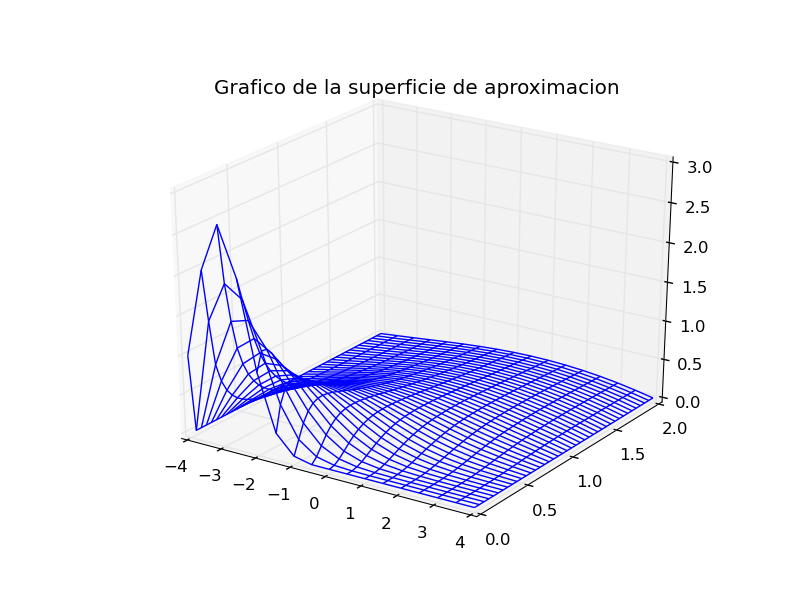
\includegraphics[scale=0.4]{p2_1}%
  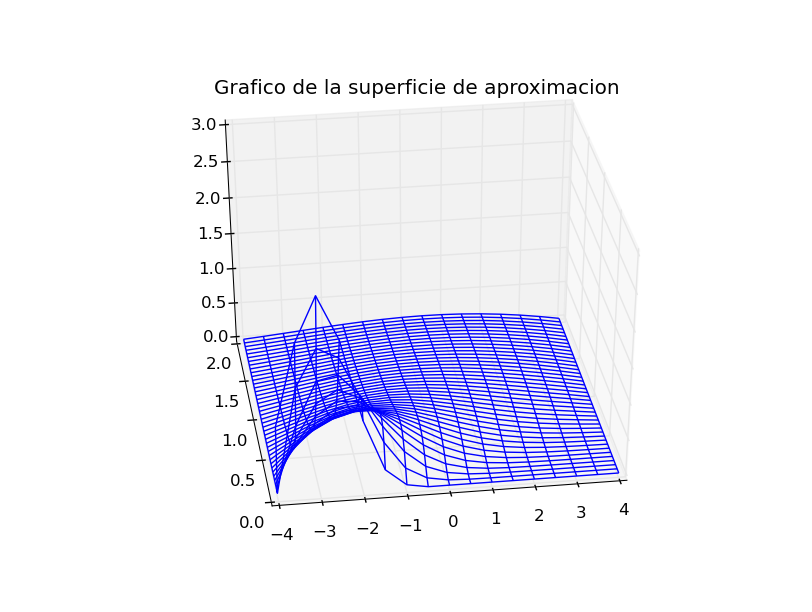
\includegraphics[scale=0.4]{p2_2}%
}%
\end{center}
\item[c)] La función de advección y difusión modela el fenómeno físico donde las partículas o la energía se transforman dentro de un sistema físico debido a los procesos de la advección y la difusión. \\[0.2cm]
El primer proceso corresponde al transporte de un fluido, o bien, a la traslación de este que produce cambios en sus propiedades. Formalmente, se define como la variación de un escalar (valor de una propiedad del fluido) producto de un campo vectorial. Un ejemplo corresponde al movimiento de las masas de aire en la atmósfera que produce cambios en su temperatura.\\[0.2cm]
Por otro lado, la difusión corresponde al proceso en el cual dos o más sustancias puestas en contacto o a través de una membrana semipermeable (o algún material con similares características) se mezclan entre sí intercambiando átomos y masa, quedando al final una mezcla completamente homogénea. Esto es más notorio en la difusión gaseosa, en donde un gas de determinadas características se mezcla y expande en el aire. \\[0.2cm]
En este caso en particular, solo se esta analizando el fenómeno en una sola dimensión, por lo que solo se estaría considerando la traslación del gas en el eje X. \\[0.2cm]
Se puede observar en el gráfico que en el tiempo $t_0$, existen altos valores de $U(x, t)$ alrededor del valor $x = -3$, el cual corresponde al valor observado de la propiedad del fluido que podría ser presión, temperatura u otro. Por otro lado, se puede notar que en aquel tiempo $t_0$, el fluido disminuye el valor de $U$ a lo largo del eje X (a medida que se aleja del punto central $x = -3$).  \\[0.2cm]
Mientras se va avanzando en el tiempo ($t > t_0$), el punto original de mayor concentración comienza rápidamente a decaer, mientras que la vecindad de dicho punto presenta leves aumentos en el valor. Esto se traduce en que, por ejemplo, un gas o un líquido como el agua, esta experimentando la difusión de su propiedad de temperatura, que inicialmente está concentrada en el punto $x = -3$, y en donde este comienza a fluir hacia el resto del líquido, hacia la derecha. \\[0.2cm]
Una vez que ha pasado un tiempo razonable (en este caso, 2 segundos), se puede notar que los valores de la propiedad son muy cercanas a cero, implicando que en esta EDP parabólica, existe una variación exponencial de la propiedad $U(x, t)$. Además, la interpretación que se da a este último comportamiento, corresponde a que la propiedad (el calor por ejemplo) se ha difundido completamente. \\[0.2cm]
Para la discretización utilizada, se debe considerar el error directo de las diferencias finitas para primeras y segundas derivadas. En primera instancia, se debe considerar la utilización de forward difference para el término $U_t$ que agrega un error de $O(\Delta t)$, luego tenemos el error que aporta el uso de central difference para aproxima el término $U_x$ que agrega un error de $O(\Delta x^2)$. Por último tenemos el error de central difference para derivada de segundo orden para aproximar el término $U_{xx}$, que aporta un error de $O(\Delta x^2)$. Por tanto, el error final del método depende de los términos $\Delta x$ y $\Delta y$ con una magnitud igual a $O(\Delta t) + 2O(\Delta x^2)$
\end{itemize}

\subsection{Parte 2: Laboratorio 4}
\begin{itemize}
\item[a)] La ecuación diferencial parcial del enunciado se puede generalizar a:
\begin{equation}
	U_{xx} + U_{yy} - \frac{1}{c^2} U_{tt} = -\frac{1}{c^2}f(t)
\end{equation}
	En donde en nuestro caso particular $f(t) = U_0 w^2 cos(wt) \delta_{i,p} \delta_{j,q}$ y $U(x,y,t)$ depende del tiempo. A continuación, multiplicando por $c^2$ a ambos lados de la ecuación y realizando un despeje del término $U_{tt}$ nos queda:
  	\begin{equation}
 		U_{tt} = c^2 ( U_{xx} + U_{yy}) + f(t)
    \end{equation}
    Haciendo uso de central difference de segundo orden para los términos $U_{xx}$, $U_{yy}$ y $U_{tt}$ y, además, realizando una discretización en donde el punto $W_{i,j,n}$ representa al punto $U(i \cdot \Delta x, j \cdot \Delta y, n \cdot \Delta t)$ a una distancia de puntos de $\Delta x$, $\Delta y$ y $\Delta t$, nos queda la siguiente ecuación:
    \begin{equation}
    \begin{split}
    	\frac{W_{i,j,n-1} - 2W_{i,j,n} + W_{i,j,n+1}}{\Delta t^2} = c^2 \left(\frac{W_{i-1,j,n} - 2W_{i,j,n} + W_{i+1,j,n}}{\Delta x^2}\right)\\ + c^2 \left(\frac{W_{i,j-1,n} - 2W_{i,j,n} + W_{i,j+1,n}}{\Delta y^2}\right) \\
        + f(t)
    \end{split}
    \end{equation}
    Despejando en la ecuación 14 el término $W_{i,j,n+1}$ que representa al punto que deseamos encontrar en el tiempo $t_{n+1}$ dado un tiempo $t_{n}$ y $t_{n-1}$, nos queda:
    \begin{equation}
    	W_{i,j,n+1} = \sigma^2 (W_{i-1,j,n} + W_{i+1,j,n} + W_{i,j-1,n} + W_{i,j+1,n}) + (2 - 4\sigma^2) W_{i,j,n} -W_{i,j,n-1} + f(t)
    \end{equation}
    Donde $\sigma = \frac{c \Delta t}{\Delta x}$. La ecuación 15 representa la discretización para la EDP, y además, la formula para encontrar los puntos en un tiempo $t_{n+1}$ dados los tiempos $t_{n}$ y $t_{n-1}$.
   \item[b)] Como se puede observar en la ecuación 15, para el tiempo $t = 0$ nos quedaría la discretización de la siguiente forma: 
   \begin{equation}
   	W_{i,j,1}= \sigma^2(W_{i-1,j,0}+W_{i+1,j,0}+W_{i,j-1,0}+W_{i,j+1,0}) + (2 - 4\sigma^2)W_{i,j,0} - W_{i,j,-1} + f(t)
   \end{equation}
   En donde el término $W_{i,j,-1}$ es necesario para poder calcular los puntos en el siguiente tiempo. Por tanto, no es posible calcular los puntos solo sabiendo las presiones en $t = 0$ y es necesario también saber las presiones en un tiempo anterior $t = -1$, el cual es mera notación y quiere decir que se necesitan dos tiempos previos antes de comenzar a calcular o realizar la simulación.
   \item[c)] Como la simulación de las ondas es un proceso costoso y, además, considerando que para mantener la estabilidad de esta se requiere que $\sigma < \frac{1}{\sqrt[]{2}}$, se han elegido como parámetros $h = 1$ y $\Delta t = 0.0001$. Se adjunta el código en el anexo. \\
   A continuación se presentan capturas de la simulación para $t = 0.0051$, $t = 0.0232$ y $t = 0.0479$ respectivamente:
   
	\begin{center}
  		\centerline{%
  			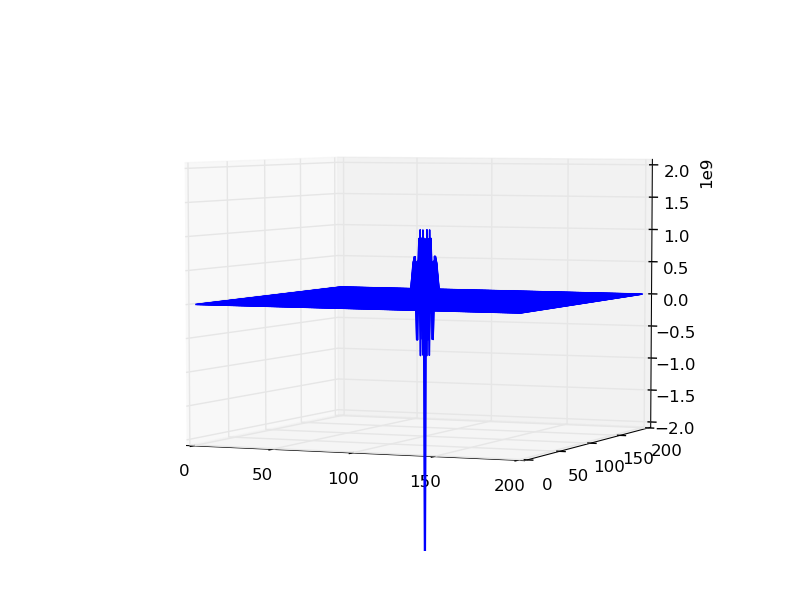
\includegraphics[scale=0.4]{lab4_t_00051}%
  			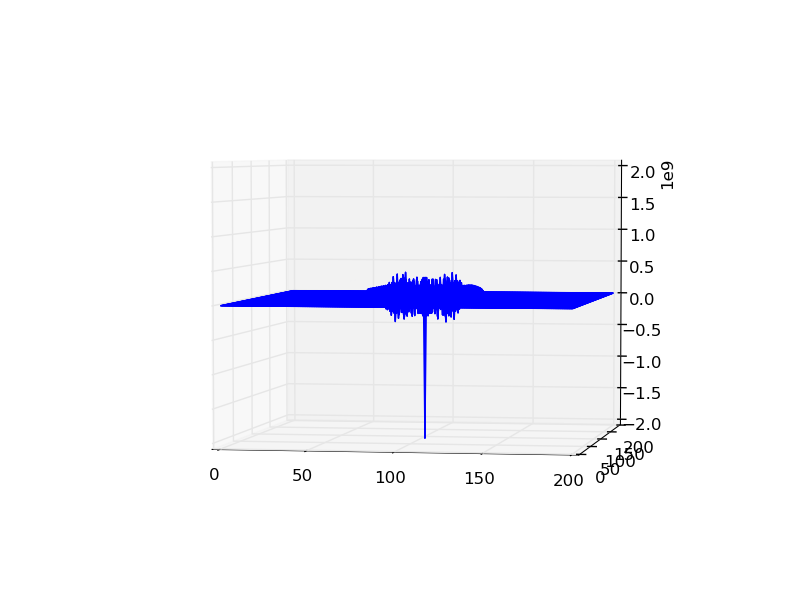
\includegraphics[scale=0.4]{lab4_t_00232}%
    	}%
        \centerline{%
        	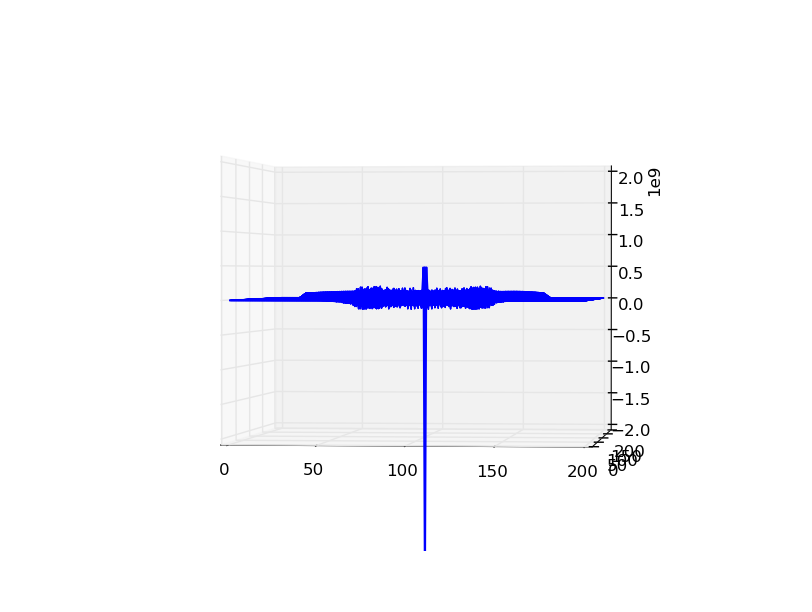
\includegraphics[scale=0.4]{lab4_t_00479}%
        }%
   \end{center}
   \item[d)] Para agregar una fuente secundaria, se debe considerar que la ecuación general para una fuente cualquiera está dada por: \\
   \begin{equation}
   	\frac{\partial^2 U}{\partial x^2} + \frac{\partial^2 U}{\partial y^2} = \frac{1}{c^2}\frac{\partial^2 U}{\partial t^2} + \frac{1}{c^2} \frac{\partial^2 U_f}{\partial t^2}
   \end{equation}
   En donde $U_f$ corresponde a la ecuación de la fuente. Es más, en la discretización de la ecuación 12, se tiene que a la derecha de la ecuación se tiene un término $f(t)$, en donde con ayuda de la funciones de Kronecker, se puede simular la posición de infinitas fuentes con distintas propiedades. \\[0.2cm]
   Basta entonces con agregar la ecuación de dicha fuente a la derecha de la ecuación, ya que la función $\delta$ (Kronecker) aseguran que la emisión de las ondas se realice desde la posición especificada en la fuente. Esto se puede generalizar para agregar infinitas fuentes de ondas.\\[0.2cm]
   Es así entonces que $f(t)$ quedaría dado por:
   \begin{equation}
   		f(t) = U_{a} w_a^2 cos(w_at)\delta_{i,p} \delta_{j,q} + U_{b} w_b^2 cos(w_bt) \delta_{i, m} \delta_{ij, n}
	\end{equation}   
   \item[e)] La simulación dará cuenta de de dos fuentes dadas por las ecuaciones $U_{a} w_a^2 cos(w_at)\delta_{i,p} \delta_{j,q}$ y $U_{b} w_b^2 cos(w_bt) \delta_{i, m} \delta_{ij, n}$, lo que permite tener dos fuentes con distintas presiones iniciales, distintas frecuencias y distintas posiciones. La fuente $A$ tendrá posición $(p, q)$, presión inicial $U_a$ y frecuencia angular $w_a$ dada su frecuencia $f_a$. La fuente $B$, tendrá posición $(m, n)$, presión inicial $U_b$ y frecuencia angular $w_b$ dada su frecuencia $f_b$. \\[0.2cm]
   El código de la simulación se encuentra disponible en el anexo. Cabe notar que la simulación requiere que $h \leq 1.0$, o de otra forma no se reconocerá la fuente en los $\delta$ Kronecker.
\end{itemize}


%\\\\\\\\\\\\\\\\\\\\\\\\\\\\\\\\\\\\\\\\\\\\\\\\\\\\
% 					CONCLUSIONES					|
%////////////////////////////////////////////////////
\newpage
\section{Conclusiones}
\subsection{Parte 1: Laboratorio 3}
\begin{itemize}
\item Las EDP elípticas no dependen del tiempo y describen la distribución de una propiedad a través de una superficie, como por ejemplo, el calor a lo largo de un plano (una superficie regular cualquiera, como una placa o mesa). Esto influye en las condiciones necesarias para resolver la EDP, en donde se requiere información en los extremos de la malla (arriba, abajo, izquierda y derecha). \\
Las EDP parabólicas dependen del tiempo y sus condiciones iniciales definen condiciones de borde a la izquierda y derecha, e información en el tiempo $t_0$ para lograr hacer evolucionar la solución.
\item Los valores de $\Delta x$, $\Delta y$ y $\Delta t$ que aparecen dependiendo del tipo de ecuación de derivadas parciales que se desee resolver, juegan un rol fundamental para generar mallas ópticas que modelan el comportamiento de EDP a través de métodos discretos, ya que definen la cantidad de puntos a utilizar y están relacionados con los errores de aproximación de los métodos. \\
Estos valores no solo especificarán el tiempo de ejecución del modelo, sino que también su precisión y fidelidad con el modelo real.

\item Los errores de aproximación que acompañan a los métodos se pueden disminuir si se disminuyen los parámetros que los acompañan. Sin embargo, a medida que estos parámetros se hacen más pequeños, se requiere un número mayor de recursos para almacenar la información, como por ejemplo, memoria requerida para almacenar los sistemas lineales y sus actualizaciones, así como también tiempo de procesador necesario para computar dichos sistemas.

\item Las condiciones iniciales son las que le dan forma a la solución final e influyen directamente en la forma final que se obtendrá graficando la malla obtenida en cada método. Como se puedo observar durante el laboratorio, a medida que nos acercamos al borde de la malla, más se parecerá la función $U(x, y)$ (o en su efecto, $U(x, t)$) a dicha condición de borde.

\item Por último, se puede notar la utilidad de los métodos finitos para resolver EDP complejas, en donde las condiciones iniciales y los valores y/o funciones que acompañan a los parámetros de las EDP permiten que se puedan modelar variados fenómenos físicos de diversas ramas e intereses, pasando por la meteorología, por la mecánica cuántica, por la electro-estática, entre varios más.
\end{itemize}
\subsection{Parte 2: Laboratorio 4}
\begin{itemize}
\item Se puede observar en la primera simulación con una sola fuente, que las ondas emitidas por la fuente se dispersan a través de todo el dominio de la malla. Esto simula como viajan las ondas sonoras a través de un medio no aislado, como por ejemplo, un parlante posicionado al centro de una habitación que envía ondas sonoras a una frecuencia determinada y fija. \\
\item En esta simulación se puede observar que si bien las ondas iniciales tienen una gran amplitud (en este caso, la amplitud se refiere a la magnitud de la presión que se ejerce a las moléculas de aire), ésta comienza lentamente a decaer a medida que se alejan de la fuente. Esto se traduce en la transferencia de energía que experimentan las ondas a medida que hacen vibrar las moléculas de aire.
\item Continuando con la primera simulación de una sola fuente, cabe notar que no existe el fenómeno de reflexión en el borde de la malla, puesto que se han dispuesto las condiciones de borde de forma de que al llegar a la frontera, las onda ya se hayan disipado.
\item En la segunda simulación, se producirá el efecto de la superposición entre las ondas generadas de la fuente $A$ y la fuente $B$, conocido también como interferencia. Esta interferencia puede se constructiva o destructiva dependiendo de los parámetros de cada fuente. En el caso de que ambas fuentes tengan los mismos parámetros, y en donde ambas fuentes tienen distintas posiciones, el tipo de interferencia dependerá de la distancia a que estas estén.
\item El error de precisión en la simulación se puede obtener considerando que se utilizó diferencias finitas para los términos $U_{xx}$, $U_{yy}$ y $U_{tt}$. Las diferencias finitas para derivadas de segundo orden corresponde a $O(\Delta x^2)$ para la segunda derivada de una función $g(x)$. Por tanto, el error final corresponde a $O(\Delta x^2)$ + $O(\Delta y^2)$ + $O(\Delta t^2)$.

\item Por último, se puede notar que la simulación implementada en la letra d) del laboratorio 4 puede ser utilizada con fuentes cualesquiera y con parámetros cualesquiera, permitiendo así simular diversos fenómenos relacionados con ondas en 2 dimensiones.
\end{itemize}

%\\\\\\\\\\\\\\\\\\\\\\\\\\\\\\\\\\\\\\\\\\\\\\\\\\\\
% 					REFERENCIAS						|
%////////////////////////////////////////////////////
\newpage
\section{Referencias}
\begin{itemize}
\item \url{https://es.wikipedia.org/wiki/Ecuaci%C3%B3n_de_convecci%C3%B3n-difusi%C3%B3n}
\item \url{http://lasmilrespuestas.blogspot.cl/2012/11/que-es-la-difusion-fisica.html}
\item \url{https://es.wikipedia.org/wiki/Convecci%C3%B3n}
\item \url{http://www.ciclohidrologico.com/adveccin}
\item \url{http://cybertesis.uach.cl/tesis/uach/2007/bmfciv344s/doc/bmfciv344s.pdf}
\end{itemize}

%\\\\\\\\\\\\\\\\\\\\\\\\\\\\\\\\\\\\\\\\\\\\\\\\\\\\
% 						ANEXO						|
%////////////////////////////////////////////////////
\newpage


\section{Anexo: Código simulación Lab 4}
\subsection{simulacion\textunderscore onda\textunderscore 3d.py}
\begin{lstlisting}[language=Python]
#!/usr/bin/env python
# -*- coding: utf-8 -*-
import math as mt
import numpy as np
import scipy as sp
from mpl_toolkits.mplot3d import Axes3D
import matplotlib.pyplot as plt
from matplotlib import cm
import pprint

def DeltaKronecker(k, m):
	if k == m:
		return 1.
	return 0.

#Retorna la siguiente matriz
#T0: Matriz en el tiempo n-1
#T1: Matriz en el tiempo n
#c: Velocidad sonido
#dt: delta t
#h: delta h
#Xmin: Minimo x
#Xmax: Maximo x
#Ymin: Minimo y
#Ymax: Maximo y
#w: Frecuencia angular
#p: Valor de p para el delta Kronecker
#q: Valor de q para el delta Kronecker
#n: numero de iteracion
#F: Function F(t)
def GetNextMatrix(T0, T1, c, dt, h, Xmin, Xmax, Ymin, Ymax, w, p, q, n, U0):
	sigma = c*dt/h
	Nx = int(mt.ceil((Xmax-Xmin)/h))
	Ny = int(mt.ceil((Ymax-Ymin)/h))

	#Inicializar siguiente matriz
	T2 = np.zeros((Ny+1, Nx+1))
	for i in xrange(0, Nx):
		for j in xrange(0, Ny):

			#Lado izquierdo
			if i == 0:
				T2[j][0] = T1[j][0] + T1[j][1] - T0[j][1] + sigma*(T1[j][1] - T1[j][0]-(T0[j][2]-T0[j][1]))

			#Lado derecho
			elif i == Nx:
				T2[j][Nx] = T1[j][Nx] + T1[j][Nx-1] - T0[j][Nx-1] + sigma*(T1[j][Nx-1] - T1[j][Nx] - (T0[j][Nx-2] - T0[j][Nx-1]))
			#Lado inferior
			elif j == 0:
				T2[0][i] = T1[0][i] + T1[1][i] - T0[1][i] + sigma*(T1[1][i] - T1[0][i] - (T0[2][i] - T0[1][i]))
			#Lado superior
			elif j == Ny:
				T2[Ny][i] = T1[Ny][i] + T1[Ny-1][i] - T0[Ny-1][i] + sigma(T1[Ny-1][i] - T1[Ny][i] - (T0[Ny-2][i] - T0[Ny-1][i]))
			#Discretizacion propia
			else:
				T2[j][i] = sigma**2*(T1[j][i-1] + T1[j][i+1] + T1[j-1][i] + T1[j+1][i]) + (2-4*sigma**2)*T1[j][i] - T0[j][i] + U0*w**2*np.cos(w*dt*n)*DeltaKronecker(i, p)*DeltaKronecker(j, q)
	return T2

#Realiza la simulacion
#f: Frecuencia f
#c: coeficiente c (velocidad del sonido)
#h: Delta x y Delta y
#dt: Deltat
#Xmin: Minimo x
#Xmax: Maximo x
#Ymin: Minimo y
#Ymax: Maximo y
#p: Posicion x de la fuente
#q: Posicion y de la fuente
#U0: Presion inicial de la fuente
def Simulacion(f, c, h, dt, Xmin, Xmax, Ymin, Ymax, p, q, U0):
	Nx = int(mt.ceil((Xmax-Xmin)/h))
	Ny = int(mt.ceil((Ymax-Ymin)/h))
	T0 = np.zeros((Ny+1, Nx+1))
	T1 = np.zeros((Ny+1, Nx+1))
	#T0 = np.full((Ny+1, Nx+1), U0)
	#T1 = np.full((Ny+1, Nx+1), U0)
	sigma = c*dt/h
	
	if(sigma >= 1/mt.sqrt(2)):
		print "Metodo inestable con el valor actual de sigma: "+str(sigma)
		return
	

	#Frecuencia angular
	w = 2*np.pi*f

	#Equiespaciado
	x = np.linspace(Xmin, Xmax, Nx+1)
	y = np.linspace(Ymin, Ymax, Ny+1)

	#Plot
	fig = plt.figure()
	ax = fig.add_subplot(111, projection='3d')
	ax.set_zlim3d(-2*10**9, 2*10**9)
	X, Y = np.meshgrid(x, y)

	max_iters = int(mt.ceil(1/dt))

	wire = ax.plot_wireframe(X, Y, T0)
	#surf = ax.plot_surface(X, Y, T0, cstride=h, rstride=h, cmap=cm.jet)

	for i in xrange(0, max_iters):
		print "t = "+str(i*dt)
		T2 = GetNextMatrix(T0, T1, c, dt, h, Xmin, Xmax, Ymin, Ymax, w, q, p, i, U0)
		T0 = T1
		T1 = T2

		wire.remove()
		#surf.remove()
		wire = ax.plot_wireframe(X, Y, T0)
		#surf = ax.plot_surface(X, Y, T0, cstride=h, rstride=h, cmap=cm.jet)
	
		plt.pause(dt)
	plt.close()


Simulacion(1000, 1500, 1, 0.0001, 0, 200, 0, 200, 100, 100, 50)
\end{lstlisting}
\subsection{simulacion2.py}
\begin{lstlisting}[language=Python]
#!/usr/bin/env python
# -*- coding: utf-8 -*-
import math as mt
import numpy as np
import scipy as sp
from mpl_toolkits.mplot3d import Axes3D
import matplotlib.pyplot as plt
from matplotlib import cm
import pprint

def DeltaKronecker(k, m):
	if k == m:
		return 1.
	return 0.

#Retorna la siguiente matriz
#T0: Matriz en el tiempo n-1
#T1: Matriz en el tiempo n
#c: Velocidad sonido
#dt: delta t
#h: delta h
#Xmin: Minimo x
#Xmax: Maximo x
#Ymin: Minimo y
#Ymax: Maximo y
#w: Frecuencia angular
#p: Valor de p para el delta Kronecker
#q: Valor de q para el delta Kronecker
#n: numero de iteracion
#F: Function F(t)
def GetNextMatrix(T0, T1, c, dt, h, Xmin, Xmax, Ymin, Ymax, wa, wb, p, q, m, n, it, Ua, Ub):
	sigma = c*dt/h
	Nx = int(mt.ceil((Xmax-Xmin)/h))
	Ny = int(mt.ceil((Ymax-Ymin)/h))

	#Inicializar siguiente matriz
	T2 = np.zeros((Ny+1, Nx+1))
	for i in xrange(0, Nx):
		for j in xrange(0, Ny):

			#Lado izquierdo
			if i == 0:
				T2[j][0] = T1[j][0] + T1[j][1] - T0[j][1] + sigma*(T1[j][1] - T1[j][0]-(T0[j][2]-T0[j][1]))

			#Lado derecho
			elif i == Nx:
				T2[j][Nx] = T1[j][Nx] + T1[j][Nx-1] - T0[j][Nx-1] + sigma*(T1[j][Nx-1] - T1[j][Nx] - (T0[j][Nx-2] - T0[j][Nx-1]))
			#Lado inferior
			elif j == 0:
				T2[0][i] = T1[0][i] + T1[1][i] - T0[1][i] + sigma*(T1[1][i] - T1[0][i] - (T0[2][i] - T0[1][i]))
			#Lado superior
			elif j == Ny:
				T2[Ny][i] = T1[Ny][i] + T1[Ny-1][i] - T0[Ny-1][i] + sigma(T1[Ny-1][i] - T1[Ny][i] - (T0[Ny-2][i] - T0[Ny-1][i]))
			#Discretizacion propia
			else:
				T2[j][i] = sigma**2*(T1[j][i-1] + T1[j][i+1] + T1[j-1][i] + T1[j+1][i]) + (2-4*sigma**2)*T1[j][i] - T0[j][i] + Ua*wa**2*np.cos(wa*dt*it)*DeltaKronecker(i, p)*DeltaKronecker(j, q) + Ub*wb**2*np.cos(wb*dt*it)*DeltaKronecker(i, m)*DeltaKronecker(j, n)
	return T2

#Realiza la simulacion
#fa: Frecuencia de la fuente A
#fb: Frecuencia de la fuente B
#c: Velocidad del sonido
#dt: Delta t
#Xmin: Minimo x
#Xmax: Maximo x
#Ymin: Minimo y
#Ymax: Maximo y
#p: Posicion x de la fuente A
#q: Posicion y de la fuente A
#m: Posicion x de la fuente B
#n: Posicion y de la fuente B
#Ua: Presion inicial de la fuente A
#Ub: Presion inicial de la fuente B
def Simulacion(fa, fb, c, h, dt, Xmin, Xmax, Ymin, Ymax, p, q, m, n, Ua, Ub):
	Nx = int(mt.ceil((Xmax-Xmin)/h))
	Ny = int(mt.ceil((Ymax-Ymin)/h))
	T0 = np.zeros((Ny+1, Nx+1))
	T1 = np.zeros((Ny+1, Nx+1))
	#T0 = np.full((Ny+1, Nx+1), U0)
	#T1 = np.full((Ny+1, Nx+1), U0)
	sigma = c*dt/h
	
	if(sigma >= 1/mt.sqrt(2)):
		print "Metodo inestable con el valor actual de sigma: "+str(sigma)
		return
	

	#Frecuencia angular
	wa = 2*np.pi*fa
	wb = 2*np.pi*fb

	#Equiespaciado
	x = np.linspace(Xmin, Xmax, Nx+1)
	y = np.linspace(Ymin, Ymax, Ny+1)

	#Plot
	fig = plt.figure()
	ax = fig.add_subplot(111, projection='3d')
	ax.set_zlim3d(-2*10**9, 2*10**9)
	X, Y = np.meshgrid(x, y)

	max_iters = int(mt.ceil(1/dt))

	wire = ax.plot_wireframe(X, Y, T0)
	#surf = ax.plot_surface(X, Y, T0, cstride=h, rstride=h, cmap=cm.jet)

	for i in xrange(0, max_iters):
		print "t = "+str(i*dt)
		T2 = GetNextMatrix(T0, T1, c, dt, h, Xmin, Xmax, Ymin, Ymax, wa, wb, p, q, m, n, i, Ua, Ub)
		T0 = T1
		T1 = T2

		wire.remove()
		#surf.remove()
		wire = ax.plot_wireframe(X, Y, T0)
		#surf = ax.plot_surface(X, Y, T0, cstride=h, rstride=h, cmap=cm.jet)
	
		plt.pause(dt)
	plt.close()

#Simulacion(fa, fb, c, h, dt, Xmin, Xmax, Ymin, Ymax, p, q, m, n, Ua, Ub):
Simulacion(1000, 1000, 1500, 1, 0.0001, 0, 200, 0, 200, 100, 100, 100, 50, 50, 50)
\end{lstlisting}
\end{document}

